\chapter{Network Security Automation e Verefoo} \label{ch:verefoo}

Nel mondo odierno le reti internet hanno rivestito un'importanza sempre maggiore, evolvendosi da piccole e semplici scenari per reti private domestiche
a grandi e complicate topologie per le aziende e la comunicazione in tutto il mondo. Trattandosi di un mondo sempre in evoluzione, anche la configurazione e
l'installazione di queste reti è diventata sempre più complessa, tanto da far notare sempre di più l'errore umano nelle impostazioni delle rete.
Per queste situazioni nasce l'idea di \textit{Network Security Automation}, che pone come obiettivo principale quello di riuscire a rendere la sicurezza delle reti
il più possibile autonoma, riducendo la possibilità di errore umano e delegando all'automatizzazione tutte le criticità della configurazione delle varie funzioni di rete.\\
In questo capitolo si introduce la definizione di \textbf{\textit{Security Function Chain (SFC)}} specificando la loro capacità nel migliorare la sicurezza delle reti,
successivamente verrà introdotto il framework Verefoo che utilizza le SFC per poter produrre delle topologie di rete robuste e sicure e automatizzare il processo di creazione e configurazione delle reti.\\
L'ultima sezione del capitolo infine spazia sugli input che il framework accetta, le \textit{Network Security Functions (NSFs)}, cioè tutte le funzioni che la rete deve rispettare come ad esempio filtrare dei pacchetti
o criptare del traffico dati. 


\section{Service Function Chain} 

All'interno delle reti è possibile far passare il traffico in maniera \textit{End-to-End, Site-to-Site o End-to-Site}.
Durante la comunicazione nelle reti moderne è solito far transitare i pacchetti attraverso nodi che si occupano di funzioni specifiche all'interno della
rete (Ad esempio un Packet Filter o un Network Address Translator NAT), che sono necessari per poter far rispettare alla rete determinate caratteristiche l'utente richiede.
I nodi che sono adibiti a svolgere le funzioni prendono il nome di \textit{Service Function (SF)} ed il collegamento di più nodi adibiti a SF viene definito 
\textit{Service Function Chain (SFC)}. Una definizione formale di SF e SFC è stata presentata nel RFC 7665 \cite{rfc7665} 
che definisce le seguenti:

\begin{itemize}
    \item \textbf{Service Function}: Una funzione che è responsabile del trattamento specifico dei pacchetti ricevuti. Una Service Function può agire su varie livelli di uno stack di protocollo (ad esempio, al livello di rete o ad altri livelli OSI). 
    Come componente logica, una SF può essere realizzata come un elemento virtuale o essere incorporata in un elemento di rete fisico.
     Una o più SF possono essere incorporate nello stesso elemento di rete. Possono esistere più occorrenze della funzione di servizio nello stesso dominio amministrativo.
    \item \textbf{Service Function Chain} Una Service Function Chain definisce un insieme ordinato di funzioni di servizio astratte e vincoli di ordinamento che devono essere applicati a pacchetti e/o frame e/o flussi selezionati come risultato di una classificazione. 
    Un esempio di una Service Function astratta è un "firewall". 
    L'ordine implicito potrebbe non essere una progressione lineare poiché l'architettura consente SFC che si ramificano su più di un percorso e consente anche casi in cui c'è flessibilità nell'ordine in cui le Service Function devono essere applicate. 
\end{itemize}

La possibilità di definire SF separate e di combinarle fra loro nell'ordine che si preferisce garantisce alle reti la possibilità di essere flessibili e scalabili facilmente.
Come infatti è descritto dalla definizione di SFC la concatenazione di più SFC permette ramificazioni su più percorsi, garantendo molteplici comunicazioni fra due host con carateristiche di sicurezza differenti.
Per comprendere meglio il concetto di SFC, un esempio fornito è il seguente:


\begin{figure}[h]  % 'h' significa che la figura viene posizionata qui
    \centering
    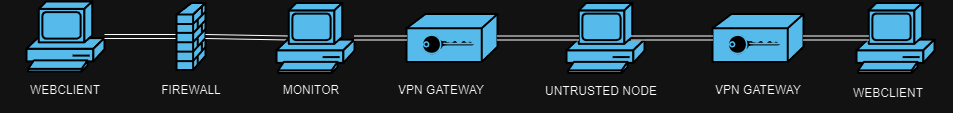
\includegraphics[width=1\textwidth]{SFC.png}  % Sostituisci 'nome_immagine' con il nome del tuo file immagine e l'estensione
    \caption{Esempio di Service Function Chain}
    \label{fig:esempio}
  \end{figure}


Come si può notare, vi sono diversi elementi all'interno di questo esempio.
Per quanto riguarda i vari SF possiamo trovare i seguenti:

\begin{itemize}
    \item \textbf{Firewall}: Si occupa di fare da packet filter fra i due webclient, per filtrare solo i pacchetti che effettivamente sono necessari alla comunicazione
    \item \textbf{Monitor}: Si occupa di monitorare il traffico in transito fra i due nodi, può essere un nodo da interrogare in caso di problematiche all'interno della rete per controllare che il firewall svolga il suo ruolo correttamente.
    \item \textbf{VPN Gateway}: Si occupa di criptare e decriptare il traffico. In questa topologia è fondamentale la loro presenza in quanto vi è un nodo considerato non affidabile, di conseguenza tutte le comunicazioni che passano attraverso quel nodo sono criptografate.
\end{itemize}

L'unione dei tre SF in questo specifico ordine definice una Service Function Chain. E' importante notare che se l'ordine fosse stato diverso (ad esempio mettendo prima i 2 VPN Gateway e dopo il firewall)
la SFC risultante sarebbe stata diversa da quella di partenza, garantendo una ramificazione.

\section{Introduzione a Verefoo}
 Il potenziamento progressivo delle tecnologie appena descritte ha portato rapidamente allo sviluppo di reti  che automatizzavano i lavori di configurazione che solitamente venivano svolti manualmente.
 Un esempio di queste nuove tecnologie viene svolto da VEREFOO\cite{Bringhenti2019}(VErified REfinement and Optimized Orchestration), un framework che si pone diversi obiettivi fra i quali la definizione
ad alto livello dei requisiti di sicurezza di rete, l'allocazione automatica ed ottimale delle varie Service Function per ottenere la maggior efficenza di rete allocando le minori risorse possibili, e la
configurazione automatica delle varie \textit{Network Security Functions}, eliminando l'errore  umano che in reti di grandi dimensioni è solito capitare.
Come è possibile intuire, la sfida di produrre una rete configurata automaticamente e correttamente è molto difficile da ottenere, perciò per assicurare la correttezza formale dei risultati ottenuti da Verefoo
l'intero framework utilizza un metodo formale che si basa sulla risoluzione di un \textit{Maximum Satisfiability Modulo Theories} (MaxSMT) tramite l'engine Z3 di Microsoft.\\
Questo, essendo basato su 3 pilastri quali \textit{Ottimizzazione, Ottimalità e Correttezza Formale}, Verefoo si pone 2 obiettivi da soddisfare:

\begin{enumerate}
    \item L'allocazione ottimale dei vari NSFs
    \item La configurazione ottimale dei vari NSFs.
\end{enumerate}

\subsection{Descrizione del modello}
Il modello di Verefoo, descritto in figura 2.2 richiede in input due elementi fondamentali:

\begin{itemize}
    \item \textbf{Service Graph}: Una topologia logica delle funzioni della rete che insieme formano un collegamento end-to-end. A differenza delle SFC il Service Graph può avere diversi percorsi per collegare due punti nella rete
    presentando la ramificazione tipica della concatenazione di SFC. Durante la creazione del Service Graph non è necessario specificare nessun requisito di sicurezza, come ad esempio Firewall, Monitors o Filtering Databases. 
    \item \textbf{Network Security Requirements}: Sono i requisiti di sicurezza che la rete in output dovrà avere dopo la computazione di Verefoo. Questo elemento è fondamentale per costruire il modello di MaxSMT da risolvere tramite Z3.
    Allo stato attuale, Verefoo consente di avere 3 requisiti di sicurezza principali:
        \begin{enumerate}
            \item \textbf{Reachability Property}: Indica che un nodo Y di destinazione deve essere raggiungibile da un nodo di partenza X in almeno un percoso della topologia.
            \item \textbf{Isolation Property}: Indica che un nodo Y di destinazione \textbf{NON} deve essere raggiungibile da un nodo di partenza X in tutti i possibili percorsi all'interno della topologia.
            \item \textbf{Protection Property}: Indica che la comunicazone tra un nodo di partenza X ed un nodo di destinazione Y deve essere sicura. In questo requisito è anche possibile specificare
                un nodo definito \textit{"Untrusted Node"} ovvero un nodo che potrebbe essere un possibile punto di debolezza nella rete e che quindi deve poter vedere solo il traffico criptografato.
        \end{enumerate}
\end{itemize}


\begin{figure}[h]  % 'h' significa che la figura viene posizionata qui
    \centering
    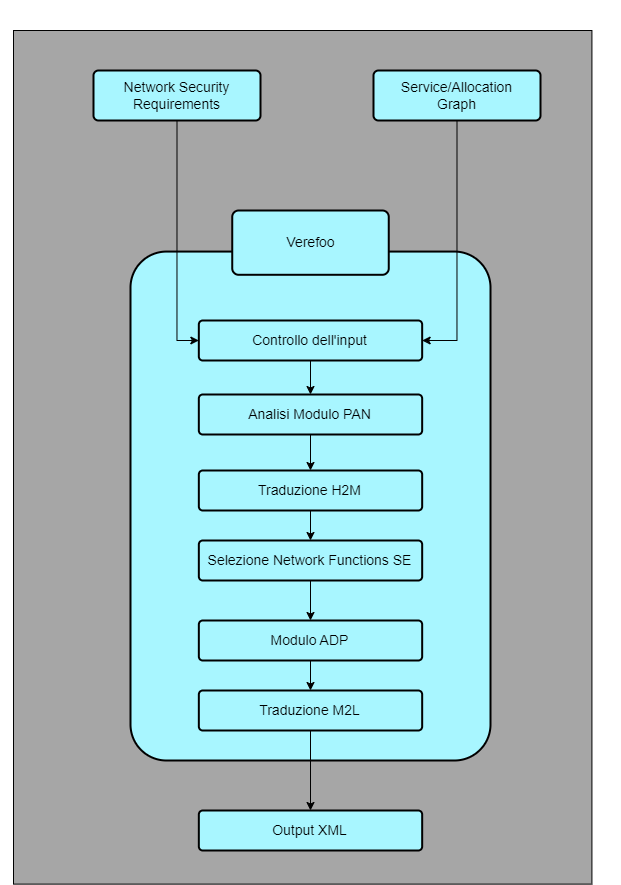
\includegraphics[width=1\textwidth]{VerefooArchitecture.png}  % Sostituisci 'nome_immagine' con il nome del tuo file immagine e l'estensione
    \caption{Architettura di VEREFOO \cite{Bringhenti2019}}
    \label{fig:esempio}
  \end{figure}

Successivamente all'input, il framework esegue una serie di passi che possono essere così riassunti:

\begin{enumerate}
    \item \textbf{Fase di controllo dell'input}: In questa fase Verefoo accetta l'input passato sotto forma di file XML e controlla la coerenza dell'input fornito. Il framework 
         oltre ad accettare l'input composto da Service Graph e NSRs accetta anche la possibilità di fornire un \textit{Allocation Graph} al posto del Service Graph(figura 2.3). La
         differenza fondamentale fra i due è che nel secondo oltre ai vari nodi della rete descritti nel Service Graph si specificano anche dei nodi aggiuntivi, chiamati \textit{Allocation Places}
         che rappresentano i punti nella topologia dove è possibile istanziare una funzione di sicurezza di rete.
    \item \textbf{Fase di analisi del modulo PAN}: qui Verefoo esegue un'analisi delle policy che sono state passate in input. Più specificatamente viene controllato che i vari NSRs siano coerenti fra
    loro, evidenziando eventuali errori (ad esempio non si può avere una Reachability Property ed una Isolation Property con gli stessi nodi di partenza e destinazione). Alla fine dell'analisi delle policy
    viene prodotto il numero minimo di vincoli che devono essere rispettati affinchè la topologia soddisfi i NSRs richiesti. In caso di errore un report viene solitamente fornito in output per comprendere 
    il perchè un determinato input non è soddisfabile.
    \item \textbf{Trasformazione a Medium Level Language}: Una volta definiti ad alto livello i vincoli da far rispettare alla topologia, questi vengono tradotti da un linguaggio di alto livello
    ad uno di medio livello tramite il componente H2M. 
    \item  \textbf{Selezione delle Network Function}:Ricevuto l'output dal modulo H2M il modulo Network Functions Selection (SE) si occupa di selezionare da un catalogo le NSF necessarie a rispettare i requisiti
    di alto e medio livello. Questo catalogo è anche accessibile al designer della rete nella fase di design disponibile nella Service GUI di Verefoo.
    \item \textbf{Allocazione, Distribuzione e Piazzamento}:Durante questo passo del framework viene eseguito, come suggerito dal titolo, l'allocazione delle varie funzioni di rete calcolate tramite
    il modulo NF Selection e i vincoli di medio livello tradotti nell'H2M. Questo compito è affidato al modulo ADP che è il cuore di Verefoo, perchè decide in quali punti della rete e con quali configurazioni
    le varie NFs devono essere allocate. L'ADP produce quindi un nuovo Service Graph nel quale sono allocate anche le funzioni di sicurezza di rete, e produce dei file di configurazione per ciascuna funzione allocata
    nel nuovo Service Graph. Queste configurazioni sono create in un linguaggio di basso livello grazie al modulo M2L presente all'interno dell'ADP.
\end{enumerate}


\begin{figure}[h]  % 'h' significa che la figura viene posizionata qui
    \centering
    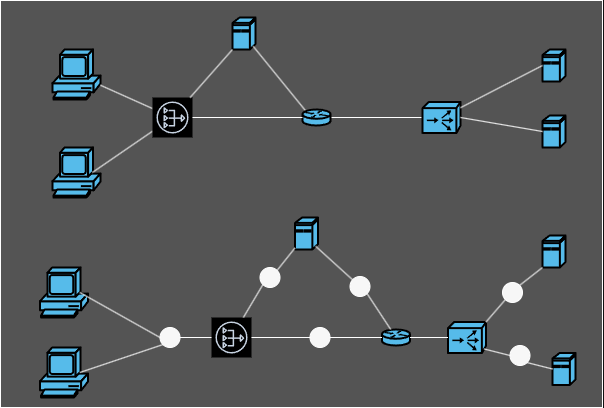
\includegraphics[width=0.9\textwidth]{Service_Allocation_Graph.png}  % Sostituisci 'nome_immagine' con il nome del tuo file immagine e l'estensione
    \caption{Esempi di Service (in alto) e Allocation(in basso) Graphs \cite{Bringhenti2019}}
    \label{fig:esempio}
  \end{figure}

\section{Definizione ed esempi delle proprietà di sicurezza}

Le proprietà di sicurezza sono il secondo input che può essere fornito a Verefoo per stabilire i vincoli necessari affinchè
si possa creare una rete sicura. A differenza del primo parametro di input, la definizione della proprietà di sicurezza è 
responsabilità dell'amministratore della rete, in quanto deve decidere tramite le possibilità offerte da Verefoo e dalla GUI ad esso associata
quante e quali proprietà inserire nella propria rete per garantire la sicurezza richiesta.\\
Per garantire flessibilità al framework è possibile inserire le definizioni sia con un linguaggio a basso livello definendo rispetti IP, porte e protocolli
da accettare o rifiutare che con un linguaggio ad alto livello nel quale i vari elementi della rete verranno definiti da dei numeri che poi saranno mappati a degli IP.

I requisiti prodotti all'interno di verefoo saranno formulati con la seguente definizione:

\begin{lstlisting}[caption={Definizione di una proprietà di sicurezza generica},float={h}]
    [ruleType, IPSrc, IPDst, portSrc, portDst, transportProto]
\end{lstlisting}

\begin{itemize}
    \item \textbf{ruleType}: specifica quale proprietà stiamo definendo. Allo stato attuale del framework ci sono 3 possibili opzione: Reachability Property, Isolation Property e Protection Property
    \item \textbf{IPSrc}: definisce da quale nodo  
    \item \textbf{IPDst}:
    \item \textbf{portSrc}:
    \item \textbf{portDst}:
    \item \textbf{transportProto}:
\end{itemize}
